\chapter{Related Work}

\section{Google Maps}
\label{Google Maps}

In March 2011, Google introduced the first indoor floorplans in their map. The intention was to increase the overview in public areas like train stations, malls and airports.
Users can upload own floorplans (valid formats include for example PNG, PDF or JPEG) to the map, with restriction to only publicly available areas.

Google Maps also offers a very popular API for their services. This allows the integration of the Google Maps Services in your own website. The usage is free for commercial use up until 28000 calls per day\footnote{According to \url{https://cloud.google.com/maps-platform/pricing/sheet/?hl=de}} and requires an API key.
The Maps JavaScript API comes with direct support for importing GeoJSON and can be customized with own content. Its designed to load maps quickly and is optimized for mobile use. Aside from that it also offers a versatile visualization library, which also includes a Heatmap Layer that helps with visualizing a heatmap (Figure 2.1.).

\begin{figure}[!hb]
	\centering
	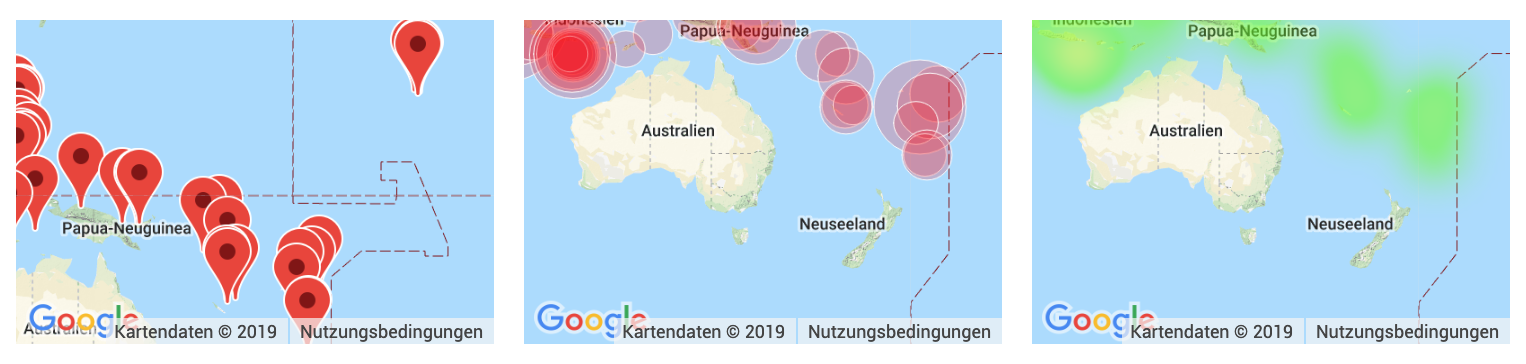
\includegraphics[width=1\linewidth]{images/GoogleMapsHeatmap}
	\caption{Example of visualization options in Google Maps}
	\label{fig:GoogleMapsHeatmap}
\end{figure}

Although this looks very promising for creating our indoor floorplan, there are quite a few problems for us.

Because the API needs an internet connection, offline development is not possible. 
Furthermore the Google Maps API would request payment after hitting the threshold of API calls mentioned above and therefore needs to be linked to an account where billing is activated. Although hitting this threshold could only happen in production, our project partner set the requirement to only use free and also open-source software and linking a billing account of our partner to use the API was not possible. 

Therefore Google Maps was not applicable to our task of creating an interactive floorplan.

\section{OpenLayers}
\label{OpenLayers}

OpenLayers is an open-source JavaScript library for displaying interactive maps. Out of the box it comes with various features like map rotation, direct mobile support and import of GeoJSON, TopoJSON, KML\footnote{Keyhole Markup Language} or GML\footnote{Geography Markup Language} data \footnote{\url{https://openlayers.org/}}. Unlike Google Maps, OpenLayers is a pure client-side library with no server-side dependencies. 

Because it has a lot of features already bundled together, it offers far more functionality than we need to meet the requirements of our floorplan. 

This also results in a heavyweight module. With a minified bundle size of 330.1 kB (Version 5.3.3) it takes up to 1.6 seconds to download on 3G\footnote{\url{https://bundlephobia.com/result?p=ol@5.3.3}}. Although this can be lowered for production by deleting unused modules, it takes extra effort to see which modules are really not used.

Due to the limited time we had for the implementation of the floorplan (due to it being the last feature on our roadmap) and only beginner knowledge of JavaScript, we needed something that is easy to understand and lets beginners output something useful in a short time. Because the abstraction layer of OpenLayers  is quite low, the learning curve can be pretty steap. Compared to Leaflet it takes a lot more code to get the same results.

Therefore we thought that OpenLayers doesn't fit our task.

\section{Leaflet}
\label{Leaflet}

Leaflet is another open-source JavaScript library for creating interactive maps. With it's first version released in 2011, it is a well established and tested library. 

By only including core features for map visualization, it only has a bundled size of 138.6KB\footnote{\url{https://bundlephobia.com/result?p=leaflet@1.5.1}}, making it a very lightweight library.

Furthermore Leaflet supports every browser and can easily be extended by plugins from the community.
This also includes plugins for creating indoor maps and real-time maps with Socket.IO. 

Considering the limited time we had for the implementation, we decided that Leaflet fits our needs the best and could be the fastest way to build our interactive live floorplan.

\section{GeoJSON}
\label{GeoJSON}

GeoJSON is a format for interchanging geospatial data and is based on JavaScript Object Notation. With the publishing of RFC 7946 in August 2016 it has a standardized format specification.
Different Geometries can be represented in a GeoJSON file. These include for example Lines, Linestrings, Polygones or Multipolygones\footnote{\url{https://tools.ietf.org/html/rfc7946}}. 

This can be used to encode the geometry for countries, houses and streets on a map, but also for encoding data for indoor rooms, stairs and hallways.

Since GeoJSON is a widely used format and supported by all major map visualization tools, including Leaflet.

\section{Socket.IO}
\label{Socket.IO}

Socket.IO is a JavaScript library that makes it possible to implement real-time applications. This is achieved through an event-based, bidirectional communication between the client and the server. 

For this to work the client-side needs to install a Socket.IO javascript library and the server needs to run a Socket.IO Node server. 

Although Socket.IO also uses WebSockets for transportation it is not an implementation of the WebSocket-protocol. It extends and combines multiple real-time protocols and switches between them if needed. Therefore a connection can only be established between a Socket.IO client and a Socket.IO server\footnote{\url{https://socket.io/docs/index.html}}.

Socket.IO offers an easy to understand API and also comes with a lot of benefits like creating realiable connections by having different fallback real-time methods, auto reconnection support and the detection of disconnections.

\section{Elastic Stack}
\label{Elastic Stack}

The Elastic Stack consists of mainly three open-source projects: \emph{Elasticsearch}, \emph{Logstash} and \emph{Kibana}.
Together they form a pipeline that can be used to analyze, search and visualize logs created from different sources. 

The component of the first stage of this pipeline is Logstash, which is responsible for collecting data from different locations and transforming it for the next step. Elasticsearch then indexes these logs and provides a RESTful API for searching. Kibana uses this API from Elasticsearch to provide meaningful visualization of the logs.
Through a smart indexing technology the Elastic Stack promises a fast response time even for large data sets and is used by companies like Netflix for monitoring security related logs or Medium for debugging production issues \footnote{\url{https://hackernoon.com/elastic-stack-a-brief-introduction-794bc7ff7d4f}}.

In our project logs sent from the gates need to be analyzed and visualized to give the FM Team more insights about the access decisions made. These informations get also displayed in the floorplan and the heatmap gets calculated based on the gate event logs. To ensure a fast display of the access decision data and to also ensure the possibility in the future to search and visualize logs not only from the gates, but from other sources also, we decided to include the Elastic Stack into our project.

